
\vspace{1cm}
\section{État de l'art}

\subsection{Introduction}

Un web Service Composite est  le résultat des différentes combinaisons de plusieurs web Services qui vise à répondre aux requêtes complexes des utilisateurs.
Pendant l'exécution des Web services composites (CWS), un Web service composant (WS) peut échouer ou tomber en panne, et pour cela il existe des stratégies qui permettent la réparation du problème telles que  la réexécution du WS,la réplication,Récupération arrière ou point de contrôle.
La question qui se pose, quelle est la meilleure stratégie de récupération ? 
Deux études existantes ont répondu a cette question en proposant des solutions pour savoir la stratégie la plus convenable (Création d’un Modèle/ Création d’un Framwork). 
Le présent chapitre décrit une présentation des web service composite avec les différentes stratégie de récupération ainsi que les deux études existantes qui répondent à notre problématique.

\subsection{Web Service Composite}

Un Web service composite est le résultat d’une composition de plusieurs Web services, et qui peut à son tour entrer dans une autre composition.
Les web services composites ont pour objectif  la production des services complexes pour répondre à des demandes d’utilisateurs complexes. 


La structure d’un Web service composite peut être générée manuellement ou automatiquement. Selon les requêtes demandées, les utilisateurs peuvent spécifier manuellement comment les fonctionnalités des Web service seront combinées ou bien  un composeur qui prend la responsabilité d’une génération automatique des Web service Composite en fonction de la demande, pour qu’ils seront finalement exécuté par un moteur d’exécution.


\begin{figure}[H]
\begin{center}
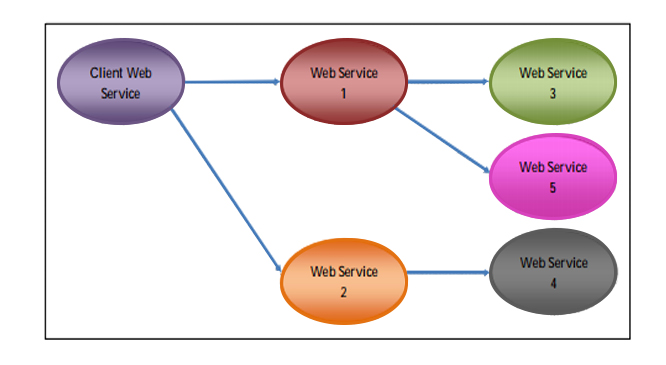
\includegraphics[width=1\linewidth]{images/CWS.jpg}
\end{center}
\caption{Web service composite}
\label{fig:1}
\end{figure}



Les Web services composite peuvent être représentés sous différents formes et structures en indiquant l’ensemble des informations et instructions relatives, comme l’ordre d’exécution et le comportement des Web services composants ainsi que les flux de données  et de contrôle.
La représentation peut être sous forme de Workflows, Graph ou réseau de Petri.



Les différents travaux et articles scientifiques sur la composition des services Web 
considèrent la composition de services Web comme étant un moyen efficace 
pour créer, exécuter, et maintenir des services qui dépendent d’autres services. Les auteurs ont défini le cycle de vie d’une composition de services Web reposant à partir de six activités [Benatalla] [Céline Lopez-Velasco] : 

- L’encapsulation de services natifs (Wrapping services): Cette première activité permet de  s’assurer que tout service peut être appelé lors d’ une composition, indépendamment de son  modèle de données, de son format de message, et de son protocole d’interaction. 


- L’établissement d’accord d’externalisation (Setting outsourcing agreements): Cette seconde activité consiste à négocier, établir, et appliquer des obligations contractuelles entre les services.


- L’assemblage de services composants (Assembling composite services):Cette activité permet  de spécifier, à un haut niveau d’abstraction, l’ensemble des services à composer afin d’atteindre  l’objectif attendu. Cet assemblage comporte une phase d’identification des services et de spécification de leurs interactions conformément aux descriptions et aux accords entre services. 


- L’exécution de services composants (Executing services):Cette activité consiste en l’exécution des spécifications de la composition précédemment définies. 


Le contrôle de l’exécution de services composites (Monitoring services): La phase de contrôle permet de superviser l’exécution de la composition en vérifiant, par exemple, l’accès aux services, les changements de statut, les échanges de messages. Ce contrôle permet de détecter des violations de contrats, de mesurer les performances des services appelés et de prédire des exceptions. 


L’évolutivité des services (Evolving services) :Cette dernière phase permet de faire évoluer la composition en modifiant les altérations de l’organisation de services, en utilisant de nouveaux  services, ou en prenant en compte les retours de la phase de contrôle. 
[Céline Lopez-Velasco]



\subsection{ Contrôle d'exécution (a voir) }



\subsection{ Tolérance aux pannes}

La tolérance aux pannes est la manière dont un système informatique, un système électronique ou un réseau répond à une défaillance matérielle ou logicielle. Le terme fait essentiellement référence à la capacité d'un système à prendre en compte les défaillances ou les dysfonctionnements d’un ou de plusieurs de ses composants, tout en fournissant un service ininterrompu, et cette capacité peut être fournie par un logiciel, un matériel ou une combinaison des deux.

Le but est d'éviter une panne catastrophique qui pourrait résulter d'un seul point de défaillance. 

\subsubsection{Défaillance des Web Service Composite}

Comme toutes les technologie, Les Web services Composite ne peuvent pas s’échapper aux défaillances d’exécution à 100 \%, car des pannes peuvent survenir à tout moment au niveau du matériel, du moteur d’exécution ou tout simplement du défaillance d’un Web service composant.
Cependant les Web Services Composite fonctionne potentiellement de manière réduite (en mode dégradé).


Soulever et relever les défis posés par les problématiques de résilience et de fiabilité des web services composite nécessite en premier lieu l’analyse  des caractéristiques des pannes dans  leur exécution.
On peut distinguer principalement dans l’environnement d’exécution des Web services Composites deux classe de pannes. 

    - Panne de nature silencieuse: (silent faults) Sont les pannes indétectables, ou qui sont détectées après une très grande durée depuis leurs déclenchements ce qui implique nécessairement que le résultat fourni est incorrect. 
    Ces pannes sont génériques pour tous les WS. Ils empêchent les WS de répondre.


    - Panne de nature logique: (Logic fault): Contrairement au pannes silencieuse, les panne logiques sont spécifiques aux différents Web service, et les attributs des entrées représente la cause principale de ces pannes.
    Ce genre d’erreur est difficile d’être identifié par le moteur d’exécution des Web services composites.

\subsubsection{Exécution tolérante aux pannes des CWS}

Le contrôle d'exécution des CWS peut être centralisé ou distribué:

- centralisé : Un seul coordinateur qui gère toute l’exécution. 
- distribué : le processus d'exécution se déroule avec la collaboration de plusieurs participants sans coordinateur central.

Le contrôle d’exécution peut être attaché aux Web Service comme il peux etre indépendant.


Certaines méthodes indépendantes de tolérance aux pannes dont apparus, telles que les propriétés transactionnelles et la réplication. Les propriétés transactionnelles décrivent implicitement le comportement des CWS en cas d'échec, et sont utilisées pour garantir la propriété transactionnelle d’atomicité.
 
\subsection{Étude 1 : Proposition d'un Modèle:}

Nous considérons: (i) que les WS peuvent subir des défaillances silencieuses (les erreurs logiques ne sont pas prises en compte); (ii) le moteur d'exécution, en charge de l'exécution du CWS, fonctionne loin des serveurs WS dans des serveurs fiables tels que les clusters, il n'échoue pas, son réseau de données est hautement sécurisé et n'est pas affecté par les fautes WS; (iii) nous supposons que l'information nécessaire pour choisir une stratégie de récupération est connue par le moteur d'exécution "à tout moment pour chaque WS. 


